\documentclass[report.tex]{subfiles}
\begin{document}
\section{Throughput for Writes (90 pts)}\label{exp4}

\subsection{Full System}

%Connect three load generating VMs to two middlewares and three memchached servers. Run a write-only experiment. 
%You need to plot throughput and response time measured on the middleware as a function of number of clients. The measurements have to be performed for 8, 16, 32 and 64 worker threads inside each middleware.
In this set of experiments, three load generating VMs are connected to a system  consisting of two middleware VMs and three server VMs running \emph{memcached}.
The number of clients is varied between 6 and 384 and the performance of a write-only workload is evaluated for configurations with 8, 16, 32 and 64 worker-threads per MW. The details of the configuration are shown in the table below.


\begin{center}
	\scriptsize{
		\begin{tabular}{|l|c|}
			\hline Number of servers                & 3          \\ 
			\hline Number of client machines        & 3          \\ 
			\hline Instances of memtier per machine & 2          \\ 
			\hline Threads per memtier instance     & 1          \\
			\hline Virtual clients per thread       & [1, 2, 4, 8, 12, 16, 24, 32, 48, 64]    \\ 
			\hline Workload                         & Write-only \\
			%\hline Multi-Get behavior               & N/A        \\
			%\hline Multi-Get size                   & N/A        \\
			\hline Number of middlewares            & 2          \\
			\hline Worker threads per middleware    & [8, 16, 32, 64]    \\
			\hline Repetitions                      & 3 or more (at least 1 minute each)  \\ 
			\hline 
		\end{tabular}
	} 
\end{center}

Table \ref{exp41_ilaw} shows that the interactive law holds for all measurements shown in this set of experiments. As previously stated the small differences in response time are a result of small throughput measurement differences between client and middleware that are within a tolerance.


\begin{table}[H]
	\scriptsize{
		\centering
		\setlength{\tabcolsep}{4.5pt}
		\begin{tabular}{|cr|*{10}{r}|}
			\cline{3-12}
			\multicolumn{2}{c|}{} & \multicolumn{10}{c|}{number of clients} \Tstrut\\
			\multicolumn{2}{c|}{} & 6 & 12 & 24 & 48 & 72 & 96 & 144 & 192 & 288 & 384 \\
			\hline
			\parbox[t]{2mm}{\multirow{4}{*}{\rotatebox[origin=c]{90}{worker}}} & 8 & -0.1 & 0.0 & 0.0 & 0.1 & 0.1 & 0.3 & 0.7 & 1.0 & 1.6 & 1.8\Tstrut\\
			& 16 & -0.1 & -0.1 & 0.0 & 0.0 & 0.1 & 0.0 & 0.4 & 0.2 & 1.0 & 2.7 \\
			& 32 & -0.1 & -0.1 & 0.0 & 0.0 & 0.0 & 0.1 & 0.2 & 0.4 & 0.7 & 0.5 \\
			& 64 & -0.1 & -0.1 & 0.0 & 0.0 & 0.1 & 0.1 & 0.2 & 0.3 & 0.3 & 0.9 \\
			& & \multicolumn{10}{c|}{in milliseconds} \\
			\hline
			\multicolumn{2}{c}{} & \multicolumn{10}{c}{write-only} \Tstrut\\ 
		\end{tabular}
		\caption{Interactive law response time deviations in milliseconds from client measurements in the full system according to equation \ref{ilaw}.}\label{exp41_ilaw}
	}
\end{table}



\begin{figure}[H]
	\begin{subfigure}[b]{.49\linewidth}
		\centering
		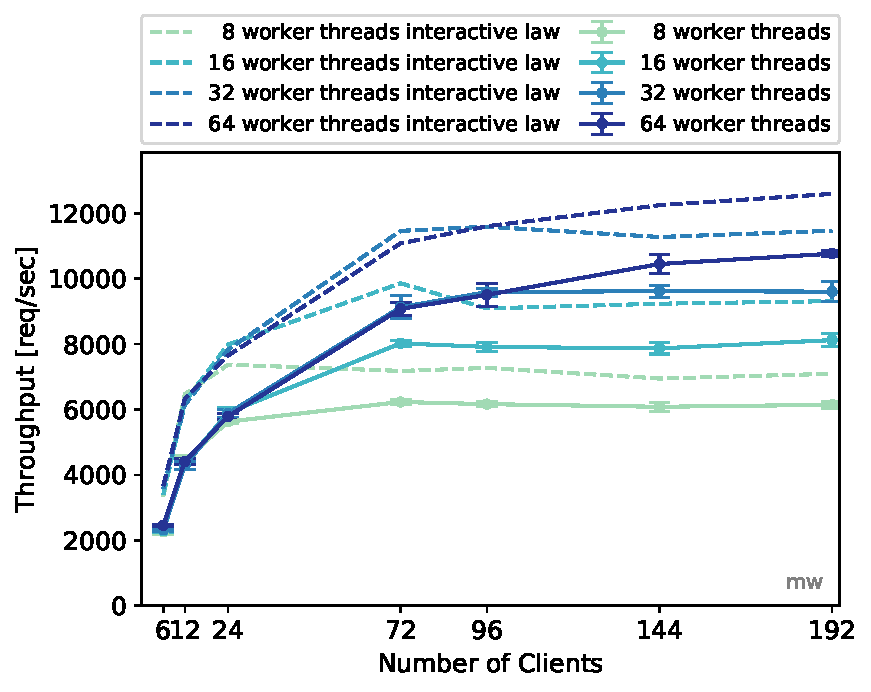
\includegraphics[width=\linewidth]{data/exp41_wo_tp_nc_w.pdf}
	\end{subfigure}\hfill
	\begin{subfigure}[b]{.49\linewidth}
		\centering
		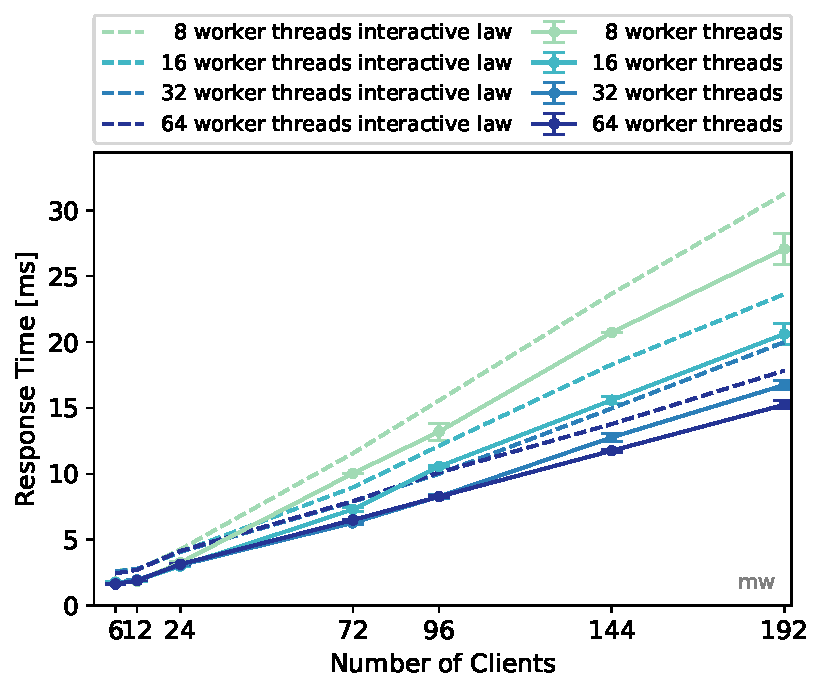
\includegraphics[width=\linewidth]{data/exp41_wo_rt_nc_w.pdf}
	\end{subfigure}%
	\caption{Throughput and response time in a write-only workload in the full system with different number of worker-threads per middleware as a function of the number of clients. Both graphs show the sample standard deviation of the measurements over the repetitions as an error metric.}\label{exp41_tp_rt_nc}
\end{figure}



\subsubsection{Explanation}

As shown in figure \ref{exp41_tp_rt_nc} the number of worker-threads heavily influences the throughput of the full system. This is consistent with the results from the MW baseline in section \ref{exp32}.
However the maximal throughput of the full system with three servers is considerably smaller than the maximal throughput from the baseline using only a single server VM. This is because a SET request relies on the response from all three servers and so the server taking the longest time determines the server service time of the request.
The effect is amplified because despite the fact that all server VMs are running with the exact same configuration, the service time of server 2 is considerably longer across all experiments than the service time of server 1 and 3 (Fig. \ref{exp41_sst_detail_nc}). This is due to the placement of the VMs in the cloud. 
In consequence the faster service times of server 1 and 3 are almost irrelevant because for most SET requests the performance of server 2 determines the service time.

The bottleneck of the system is the number of worker-threads waiting for the slowest server to respond.
This becomes evident when considering the utilization of the different components of the system in figure \ref{exp41_util_nc}. This also explains why the throughput for different number of workers saturates for a different number of clients.

The server service time is increasing in the number of clients up to the point where all worker-threads are almost constantly busy and remains more or less constant from there (Fig. \ref{exp41_sst_detail_nc}) because the number of worker-threads puts a limit on the maximal load a server VM incurs. At the point where all worker-threads are constantly busy, incoming decoded requests need to wait in the queue. These two effects combined lead to an increasing response time in the number of clients as shown in figure \ref{exp41_tp_rt_nc}. This mechanism was already analysed in detail in the MW baseline section \ref{exp3}.


\begin{figure}[H]
	\begin{subfigure}[b]{.49\linewidth}
		\centering
		\includegraphics[width=\linewidth]{data/exp41_util_nc_w8.pdf}
		\caption{8 worker-threads}
	\end{subfigure}\hfill
	\begin{subfigure}[b]{.49\linewidth}
		\centering
		\includegraphics[width=\linewidth]{data/exp41_util_nc_w64.pdf}
		\caption{64 worker-threads}
	\end{subfigure}%
	\caption{Component utilization}\label{exp41_util_nc}
\end{figure}


\begin{figure}[H]
	\begin{subfigure}[b]{.49\linewidth}
		\centering
		\includegraphics[width=\linewidth]{data/exp41_sst_detail_nc_w8.pdf}
		\caption{8 worker-threads}
	\end{subfigure}\hfill
	\begin{subfigure}[b]{.49\linewidth}
		\centering
		\includegraphics[width=\linewidth]{data/exp41_sst_detail_nc_w64.pdf}
		\caption{64 worker-threads}
	\end{subfigure}%
	\caption{Server service time per server}\label{exp41_sst_detail_nc}
\end{figure}


\subsection{Summary}

%Based on the experiments above, fill out the following table with the data corresponding to the maximum throughput point for all four worker-thread scenarios.

\begin{center}
	{Maximum throughput for the full system}
	\begin{tabular}{|l|p{1.5cm}|p{1.5cm}|p{1.5cm}|p{1.5cm}|}
		\hline                                            			& WT=8 & WT=16 & WT=32 & WT=64 \\ 
		\hline Throughput [ops/sec] (Middleware)                    & 6262 &  8102 & 10154 & 11206 \\ 
		\hline Throughput [ops/sec] & 6057 &  8081 & 10186 & 11562 \\ 
		(Derived from MW response time) &  &   &  &  \\ 
		\hline Throughput [ops/sec] (Client)              			& 6389 &  8250 & 10242 & 11391 \\ 
		\hline Average time in queue [ms]                 			&  4.0 &   3.6 &   2.1 &   1.3 \\ 
		\hline Average length of queue                    			&   12 &    15 &    11 &     8 \\ 
		\hline Average time waiting for memcached [ms]    			&  2.4 &   3.7 &   5.7 &   9.6 \\ 
		\hline 
	\end{tabular}
\end{center}

%Based on the data provided in these tables, draw conclusions on the state of your system for a variable number of worker threads.
\paragraph{Throughput}
The maximum throughput with 8 worker-threads is reached with 48 clients, for 16 worker-threads with 72 clients, for 32 worker-threads with 96 clients and for 64 worker-threads with 144 clients.
 
As described in section \ref{exp2} the interactive law\footnote{In a closed system with $N$ clients the throughput $X$ can be derived using the response time $R$ and the client thinking time $Z$} $X = \frac{N}{R+Z}$ cannot be applied directly when using the middleware response time because it does not include the time to transfer the request and the response between client VM and middleware VM. To overcome this issue the estimate of the round trip time measured before the set of experiments is used as client thinking time $Z$. This is a sensible choice because in the viewpoint of the middleware the next request arrives not before the response of the previous request arrived at the client VM and the new request was transferred to the middleware VM and so it appears as if the client is waiting for this time.
The deviations between measured throughput in the middleware and derived throughput from middleware response time is explained by the fact that the round trip time is only an estimate and the cloud is not an isolated environment and so the network performance varies over time. In particular for smaller number of clients and shorter response times, errors in the estimate lead to slightly bigger differences.
The deviations between middleware and client throughput measurements are consistent with the differences observed in other experiments, but overall the differences are not significant.


\paragraph{Number of Worker-Threads}
The collected data clearly shows that a larger number of worker-threads lead to a higher throughput because a worker-thread is blocked waiting for all server responses to return and so adding additional worker-threads leads to more concurrency in the system. Consequently for the same number of clients, requests spend less time in the queue which outweights the negative effect that the average time waiting for memcached increases in the number of worker-threads.

In the configuration with maximal throughput the queue is always small because otherwise the average time spent in the queue would lead to a significantly longer response time without much benefit in terms of throughput because already in the current state worker-threads are working almost all the time. 


\paragraph{Key take-away messages}
\begin{itemize}
	\vitemsep
	\item for each SET request, the slowest server determines the server service time. Hence the performance of the system with a single server cannot be reached.
	\item placement of server VM important factor for performance
	\item number of worker-threads is important factor for performance
\end{itemize}

\end{document}